% Created by tikzDevice version 0.12 on 2018-09-28 04:16:53
% !TEX encoding = UTF-8 Unicode
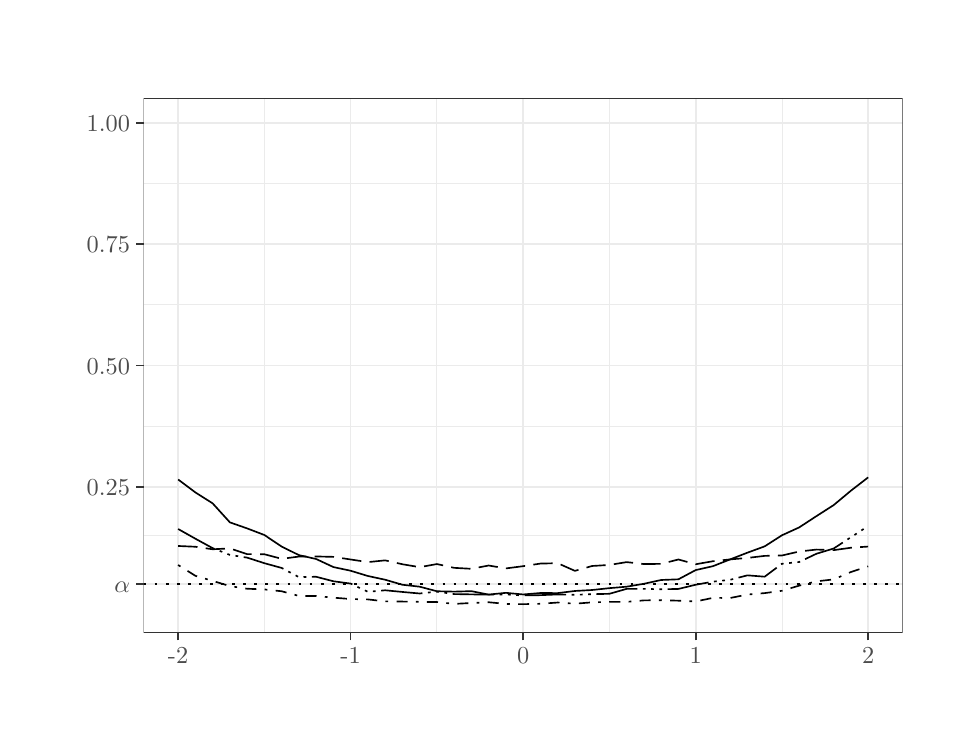
\begin{tikzpicture}[x=1pt,y=1pt]
\definecolor{fillColor}{RGB}{255,255,255}
\path[use as bounding box,fill=fillColor,fill opacity=0.00] (0,0) rectangle (325.21,252.94);
\begin{scope}
\path[clip] (  0.00,  0.00) rectangle (325.21,252.94);
\definecolor{drawColor}{RGB}{255,255,255}
\definecolor{fillColor}{RGB}{255,255,255}

\path[draw=drawColor,line width= 0.6pt,line join=round,line cap=round,fill=fillColor] (  0.00,  0.00) rectangle (325.21,252.94);
\end{scope}
\begin{scope}
\path[clip] ( 41.90, 34.26) rectangle (316.18,227.38);
\definecolor{fillColor}{RGB}{255,255,255}

\path[fill=fillColor] ( 41.90, 34.26) rectangle (316.18,227.38);
\definecolor{drawColor}{gray}{0.92}

\path[draw=drawColor,line width= 0.3pt,line join=round] ( 41.90, 69.37) --
	(316.18, 69.37);

\path[draw=drawColor,line width= 0.3pt,line join=round] ( 41.90,108.87) --
	(316.18,108.87);

\path[draw=drawColor,line width= 0.3pt,line join=round] ( 41.90,152.76) --
	(316.18,152.76);

\path[draw=drawColor,line width= 0.3pt,line join=round] ( 41.90,196.65) --
	(316.18,196.65);

\path[draw=drawColor,line width= 0.3pt,line join=round] ( 85.53, 34.26) --
	( 85.53,227.38);

\path[draw=drawColor,line width= 0.3pt,line join=round] (147.87, 34.26) --
	(147.87,227.38);

\path[draw=drawColor,line width= 0.3pt,line join=round] (210.21, 34.26) --
	(210.21,227.38);

\path[draw=drawColor,line width= 0.3pt,line join=round] (272.55, 34.26) --
	(272.55,227.38);

\path[draw=drawColor,line width= 0.6pt,line join=round] ( 41.90, 51.81) --
	(316.18, 51.81);

\path[draw=drawColor,line width= 0.6pt,line join=round] ( 41.90, 86.93) --
	(316.18, 86.93);

\path[draw=drawColor,line width= 0.6pt,line join=round] ( 41.90,130.82) --
	(316.18,130.82);

\path[draw=drawColor,line width= 0.6pt,line join=round] ( 41.90,174.71) --
	(316.18,174.71);

\path[draw=drawColor,line width= 0.6pt,line join=round] ( 41.90,218.60) --
	(316.18,218.60);

\path[draw=drawColor,line width= 0.6pt,line join=round] ( 54.37, 34.26) --
	( 54.37,227.38);

\path[draw=drawColor,line width= 0.6pt,line join=round] (116.70, 34.26) --
	(116.70,227.38);

\path[draw=drawColor,line width= 0.6pt,line join=round] (179.04, 34.26) --
	(179.04,227.38);

\path[draw=drawColor,line width= 0.6pt,line join=round] (241.38, 34.26) --
	(241.38,227.38);

\path[draw=drawColor,line width= 0.6pt,line join=round] (303.71, 34.26) --
	(303.71,227.38);
\definecolor{drawColor}{RGB}{0,0,0}

\path[draw=drawColor,line width= 0.6pt,dash pattern=on 1pt off 3pt on 4pt off 3pt ,line join=round] ( 54.37, 58.77) --
	( 60.60, 54.87) --
	( 66.83, 53.04) --
	( 73.07, 51.15) --
	( 79.30, 50.20) --
	( 85.53, 49.95) --
	( 91.77, 49.29) --
	( 98.00, 47.60) --
	(104.24, 47.57) --
	(110.47, 46.97) --
	(116.70, 46.48) --
	(122.94, 46.34) --
	(129.17, 45.63) --
	(135.40, 45.56) --
	(141.64, 45.46) --
	(147.87, 45.39) --
	(154.10, 44.72) --
	(160.34, 45.04) --
	(166.57, 45.32) --
	(172.81, 44.72) --
	(179.04, 44.62) --
	(185.27, 44.76) --
	(191.51, 45.21) --
	(197.74, 44.79) --
	(203.97, 45.28) --
	(210.21, 45.46) --
	(216.44, 45.46) --
	(222.68, 45.99) --
	(228.91, 46.06) --
	(235.14, 45.88) --
	(241.38, 45.60) --
	(247.61, 46.90) --
	(253.84, 46.86) --
	(260.08, 48.09) --
	(266.31, 48.62) --
	(272.55, 49.46) --
	(278.78, 51.32) --
	(285.01, 52.87) --
	(291.25, 53.57) --
	(297.48, 56.24) --
	(303.71, 58.28);

\path[draw=drawColor,line width= 0.6pt,dash pattern=on 15pt off 2pt on 1pt off 2pt on 1pt off 2pt on 1pt off 2pt ,line join=round] ( 54.37, 71.79) --
	( 60.60, 68.28) --
	( 66.83, 64.88) --
	( 73.07, 62.42) --
	( 79.30, 61.44) --
	( 85.53, 59.43) --
	( 91.77, 57.71) --
	( 98.00, 54.41) --
	(104.24, 54.52) --
	(110.47, 52.90) --
	(116.70, 52.06) --
	(122.94, 49.08) --
	(129.17, 49.64) --
	(135.40, 49.04) --
	(141.64, 48.48) --
	(147.87, 49.15) --
	(154.10, 48.27) --
	(160.34, 48.16) --
	(166.57, 48.06) --
	(172.81, 48.13) --
	(179.04, 47.78) --
	(185.27, 47.88) --
	(191.51, 48.13) --
	(197.74, 47.99) --
	(203.97, 48.23) --
	(210.21, 48.37) --
	(216.44, 50.16) --
	(222.68, 50.16) --
	(228.91, 49.99) --
	(235.14, 50.13) --
	(241.38, 51.64) --
	(247.61, 52.76) --
	(253.84, 53.43) --
	(260.08, 55.04) --
	(266.31, 54.55) --
	(272.55, 59.22) --
	(278.78, 59.86) --
	(285.01, 62.84) --
	(291.25, 64.74) --
	(297.48, 68.81) --
	(303.71, 72.85);

\path[draw=drawColor,line width= 0.6pt,dash pattern=on 7pt off 3pt ,line join=round] ( 54.37, 65.65) --
	( 60.60, 65.37) --
	( 66.83, 64.46) --
	( 73.07, 64.77) --
	( 79.30, 62.70) --
	( 85.53, 62.66) --
	( 91.77, 61.01) --
	( 98.00, 61.82) --
	(104.24, 61.86) --
	(110.47, 61.72) --
	(116.70, 60.77) --
	(122.94, 59.82) --
	(129.17, 60.45) --
	(135.40, 59.05) --
	(141.64, 57.99) --
	(147.87, 59.12) --
	(154.10, 57.75) --
	(160.34, 57.40) --
	(166.57, 58.59) --
	(172.81, 57.54) --
	(179.04, 58.35) --
	(185.27, 59.29) --
	(191.51, 59.43) --
	(197.74, 56.66) --
	(203.97, 58.42) --
	(210.21, 58.80) --
	(216.44, 59.82) --
	(222.68, 59.12) --
	(228.91, 59.19) --
	(235.14, 60.77) --
	(241.38, 59.05) --
	(247.61, 60.14) --
	(253.84, 60.80) --
	(260.08, 61.33) --
	(266.31, 62.07) --
	(272.55, 62.21) --
	(278.78, 63.65) --
	(285.01, 64.35) --
	(291.25, 64.14) --
	(297.48, 65.02) --
	(303.71, 65.44);

\path[draw=drawColor,line width= 0.6pt,line join=round] ( 54.37, 89.67) --
	( 60.60, 85.00) --
	( 66.83, 81.06) --
	( 73.07, 74.18) --
	( 79.30, 72.00) --
	( 85.53, 69.62) --
	( 91.77, 65.44) --
	( 98.00, 62.35) --
	(104.24, 60.94) --
	(110.47, 58.03) --
	(116.70, 56.70) --
	(122.94, 54.80) --
	(129.17, 53.46) --
	(135.40, 51.64) --
	(141.64, 50.94) --
	(147.87, 49.29) --
	(154.10, 49.15) --
	(160.34, 49.32) --
	(166.57, 48.09) --
	(172.81, 48.72) --
	(179.04, 48.13) --
	(185.27, 48.65) --
	(191.51, 48.62) --
	(197.74, 49.39) --
	(203.97, 49.74) --
	(210.21, 50.41) --
	(216.44, 50.94) --
	(222.68, 51.99) --
	(228.91, 53.36) --
	(235.14, 53.61) --
	(241.38, 56.94) --
	(247.61, 58.35) --
	(253.84, 60.80) --
	(260.08, 63.23) --
	(266.31, 65.51) --
	(272.55, 69.51) --
	(278.78, 72.36) --
	(285.01, 76.43) --
	(291.25, 80.43) --
	(297.48, 85.63) --
	(303.71, 90.44);

\path[draw=drawColor,line width= 0.6pt,dash pattern=on 1pt off 3pt ,line join=round] ( 41.90, 51.81) -- (316.18, 51.81);
\definecolor{drawColor}{gray}{0.20}

\path[draw=drawColor,line width= 0.6pt,line join=round,line cap=round] ( 41.90, 34.26) rectangle (316.18,227.38);
\end{scope}
\begin{scope}
\path[clip] (  0.00,  0.00) rectangle (325.21,252.94);
\definecolor{drawColor}{gray}{0.30}

\node[text=drawColor,anchor=base east,inner sep=0pt, outer sep=0pt, scale=  0.88] at ( 36.95, 48.78) {$\alpha$};

\node[text=drawColor,anchor=base east,inner sep=0pt, outer sep=0pt, scale=  0.88] at ( 36.95, 83.90) {$0.25$};

\node[text=drawColor,anchor=base east,inner sep=0pt, outer sep=0pt, scale=  0.88] at ( 36.95,127.79) {$0.50$};

\node[text=drawColor,anchor=base east,inner sep=0pt, outer sep=0pt, scale=  0.88] at ( 36.95,171.68) {$0.75$};

\node[text=drawColor,anchor=base east,inner sep=0pt, outer sep=0pt, scale=  0.88] at ( 36.95,215.57) {$1.00$};
\end{scope}
\begin{scope}
\path[clip] (  0.00,  0.00) rectangle (325.21,252.94);
\definecolor{drawColor}{gray}{0.20}

\path[draw=drawColor,line width= 0.6pt,line join=round] ( 39.15, 51.81) --
	( 41.90, 51.81);

\path[draw=drawColor,line width= 0.6pt,line join=round] ( 39.15, 86.93) --
	( 41.90, 86.93);

\path[draw=drawColor,line width= 0.6pt,line join=round] ( 39.15,130.82) --
	( 41.90,130.82);

\path[draw=drawColor,line width= 0.6pt,line join=round] ( 39.15,174.71) --
	( 41.90,174.71);

\path[draw=drawColor,line width= 0.6pt,line join=round] ( 39.15,218.60) --
	( 41.90,218.60);
\end{scope}
\begin{scope}
\path[clip] (  0.00,  0.00) rectangle (325.21,252.94);
\definecolor{drawColor}{gray}{0.20}

\path[draw=drawColor,line width= 0.6pt,line join=round] ( 54.37, 31.51) --
	( 54.37, 34.26);

\path[draw=drawColor,line width= 0.6pt,line join=round] (116.70, 31.51) --
	(116.70, 34.26);

\path[draw=drawColor,line width= 0.6pt,line join=round] (179.04, 31.51) --
	(179.04, 34.26);

\path[draw=drawColor,line width= 0.6pt,line join=round] (241.38, 31.51) --
	(241.38, 34.26);

\path[draw=drawColor,line width= 0.6pt,line join=round] (303.71, 31.51) --
	(303.71, 34.26);
\end{scope}
\begin{scope}
\path[clip] (  0.00,  0.00) rectangle (325.21,252.94);
\definecolor{drawColor}{gray}{0.30}

\node[text=drawColor,anchor=base,inner sep=0pt, outer sep=0pt, scale=  0.88] at ( 54.37, 23.25) {-2};

\node[text=drawColor,anchor=base,inner sep=0pt, outer sep=0pt, scale=  0.88] at (116.70, 23.25) {-1};

\node[text=drawColor,anchor=base,inner sep=0pt, outer sep=0pt, scale=  0.88] at (179.04, 23.25) {0};

\node[text=drawColor,anchor=base,inner sep=0pt, outer sep=0pt, scale=  0.88] at (241.38, 23.25) {1};

\node[text=drawColor,anchor=base,inner sep=0pt, outer sep=0pt, scale=  0.88] at (303.71, 23.25) {2};
\end{scope}
\end{tikzpicture}
